\documentclass[letterpaper,12pt]{article}
\usepackage{array}
\usepackage{threeparttable}
\usepackage{geometry}
\geometry{letterpaper,tmargin=1in,bmargin=1in,lmargin=1.25in,rmargin=1.25in}
\usepackage{fancyhdr,lastpage}
\pagestyle{fancy}
\lhead{}
\chead{}
\rhead{}
\lfoot{}
\cfoot{}
\rfoot{\footnotesize\textsl{Page \thepage\ of \pageref{LastPage}}}
\renewcommand\headrulewidth{0pt}
\renewcommand\footrulewidth{0pt}
\usepackage[format=hang,font=normalsize,labelfont=bf]{caption}
\usepackage{listings}
\lstset{frame=single,
  language=Python,
  showstringspaces=false,
  columns=flexible,
  basicstyle={\small\ttfamily},
  numbers=none,
  breaklines=true,
  breakatwhitespace=true
  tabsize=3
}
\usepackage{amsmath}
\usepackage{amssymb}
\usepackage{amsthm}
\usepackage{harvard}
\usepackage{setspace}
\usepackage{float,color}
\usepackage[pdftex]{graphicx}
\usepackage{hyperref}
\hypersetup{colorlinks,linkcolor=red,urlcolor=blue}
\theoremstyle{definition}
\newtheorem{theorem}{Theorem}
\newtheorem{acknowledgement}[theorem]{Acknowledgement}
\newtheorem{algorithm}[theorem]{Algorithm}
\newtheorem{axiom}[theorem]{Axiom}
\newtheorem{case}[theorem]{Case}
\newtheorem{claim}[theorem]{Claim}
\newtheorem{conclusion}[theorem]{Conclusion}
\newtheorem{condition}[theorem]{Condition}
\newtheorem{conjecture}[theorem]{Conjecture}
\newtheorem{corollary}[theorem]{Corollary}
\newtheorem{criterion}[theorem]{Criterion}
\newtheorem{definition}[theorem]{Definition}
\newtheorem{derivation}{Derivation} % Number derivations on their own
\newtheorem{example}[theorem]{Example}
\newtheorem{exercise}[theorem]{Exercise}
\newtheorem{lemma}[theorem]{Lemma}
\newtheorem{notation}[theorem]{Notation}
\newtheorem{problem}[theorem]{Problem}
\newtheorem{proposition}{Proposition} % Number propositions on their own
\newtheorem{remark}[theorem]{Remark}
\newtheorem{solution}[theorem]{Solution}
\newtheorem{summary}[theorem]{Summary}
%\numberwithin{equation}{section}
\bibliographystyle{aer}
\newcommand\ve{\varepsilon}
\newcommand\boldline{\arrayrulewidth{1pt}\hline}


\begin{document}

\begin{flushleft}
  \textbf{\large{Problem Set \#2, Set 1}} \\
  Charlie Walker
\end{flushleft}

\vspace{5mm}

\noindent\textbf{Exercise 1}\\

The spectral radius less than 1 implies a unique solution. Using successive approximations (see code in \texttt{exercises1.py}), we find the answer converges to:

\begin{equation*}
	x =\begin{bmatrix}
		-0.89552239\\
		13.34328358\\
		45.64179105
		\end{bmatrix}
\end{equation*}
Matrix algebra confirms the result:
\begin{equation*}
\begin{split}
\begin{bmatrix}
	x_1\\
	x_2\\
	x_3
\end{bmatrix}
&=\begin{bmatrix}
	0.6 & 0.1 & -0.3 \\
	0.5 & -0.4 & 0.2 \\
	1.0 & -0.2 & 1.1 
\end{bmatrix}
\begin{bmatrix}
	x_1\\
	x_2\\
	x_3
\end{bmatrix}
+\begin{bmatrix}
	12\\
	10\\
	-1
\end{bmatrix}\\
\implies x&\approx\begin{bmatrix}
		-0.89552239\\
		13.34328358\\
		45.64179105
\end{bmatrix}
\end{split}
\end{equation*}\\

\noindent\textbf{Exercise 2}\\

Suffices to show that the equation is a contraction map. For any $x_1, x_2$,
\begin{equation*}
\begin{split}
&|c(1-\beta) + \beta\sum_{k=1}^{K}\max\{w_k,x_1\}p_k - c(1-\beta) + \beta\sum_{k=1}^{K}\max\{w_k,x_2\}p_k|\\
&=|\beta\sum_{k=1}^{K}\max\{w_k,x_1\}p_k - \beta\sum_{k=1}^{K}\max\{w_k,x_2\}p_k|\\
&=\beta|\sum_{k=1}^{K}\max\{w_k,x_1\}p_k - \sum_{k=1}^{K}\max\{w_k,x_2\}p_k|\\
&=\beta|\sum_{k=1}^{K}(\max\{w_k,x_1\} - max\{w_k, x_2\}|p_k\\
&\leq \beta\sum_{k=1}^{K}|(\max\{w_k,x_1\} - max\{w_k, x_2\}|p_k\\
&\leq \sup|\max\{w_k,x_1\} - max\{w_k, x_2\}|\\
&\leq \beta|x_1 - x_2|
\end{split}
\end{equation*}
Yes, the function is a contraction, so has  unique fixed point solution. The function applied to itself forms a Cauchy sequence that converges to the fixed point, so the unique solution can be computed by iterating over the sequence.\\

\noindent\textbf{Exercise 3}\\
See code in \texttt{exercises1.py}. Figure 1 shows the positive relationship between unemployment compensation and reservation wages, in line with intuition.\\
 
\begin{figure}[htb]\centering\captionsetup{width=4.0in}
  \caption{\textbf{Unemployment compensation and reservation wages}}\label{FigExample}
  \fbox{\resizebox{4.0in}{3.0in}{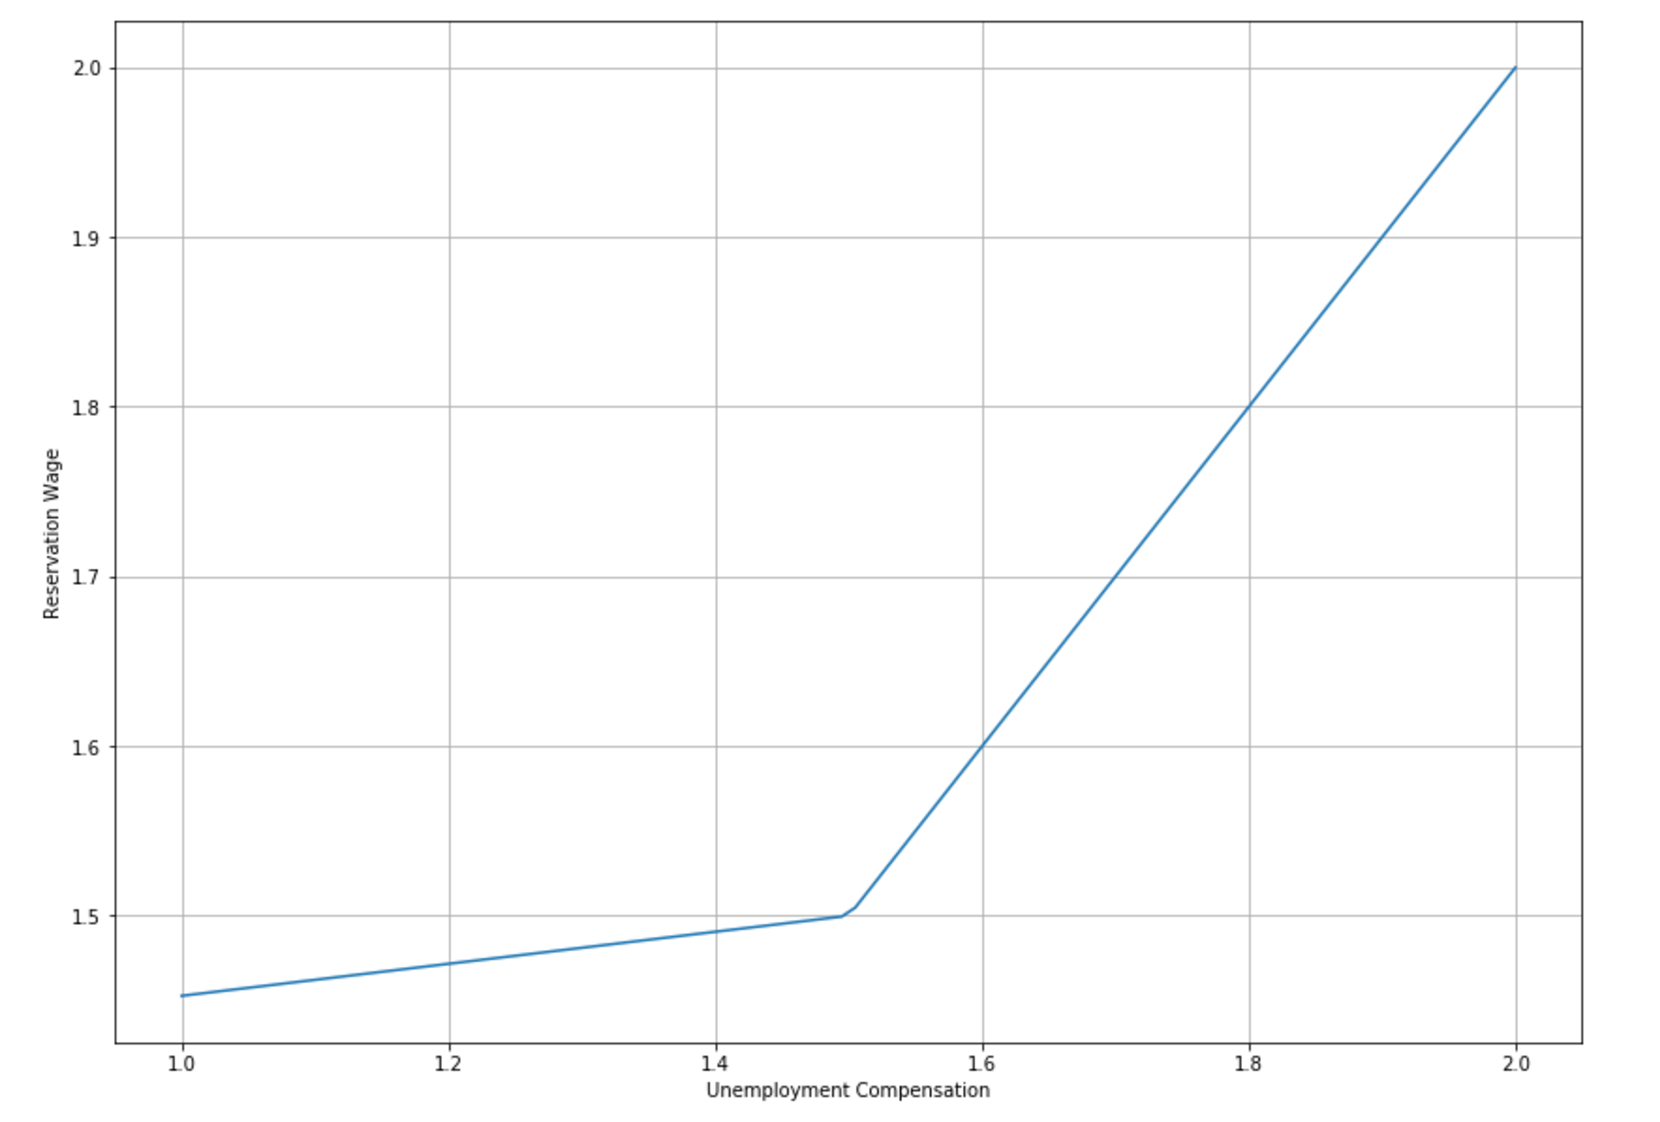
\includegraphics{reswage.png}}}
\end{figure}


\end{document}

